
\section{Interazioni fra componenti}
\label{sec:Interazioni}
\subsection{Costruzione del grafo della mappa topologica}

\begin{figure}[H]
	\centering
	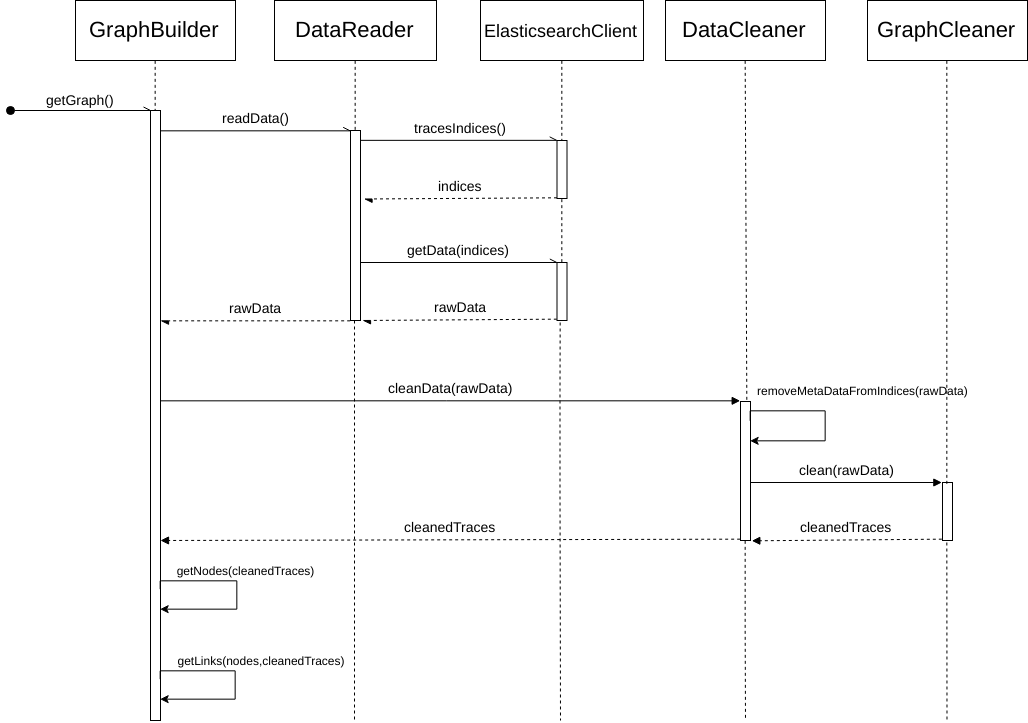
\includegraphics[width=1\textwidth]{Images/DiagrammaSequenzaGraph.png}
	\caption{Diagramma di Sequenza UML rappresentante la costruzione del grafo della mappa topologica}
	\label{img:seqGraph}
\end{figure}

Un'istanza di \texttt{GraphBuilder} richiama il metodo \texttt{readData()} su un oggetto \texttt{DataReader} che si occupa prima di selezionare gli indici dell'istanza di Elasticsearch che hanno al loro interno delle traces tramite la funzione \texttt{tracesIndices()} e successivamente di effettuare una richiesta per ogni indice recuperato al fine di recupera i dati associati.
Ricevuti i dati, viene invocato il metodo \texttt{cleanData()} passandogli come parametro i dati, che si occupa della pulizia dei dati superflui provenienti da Elasticsearch tramite la funzione \texttt{removeDataFromIndices()}. Tramite la funzione \texttt{clean()} invece vengono puliti i dati superflui alla costruzione della mappa topologica attraverso un'istanza di \texttt{GraphCleaner}.
In seguito alla pulizia dei dati, l'istanza di \texttt{GraphBuilder} costruisce l'insieme dei nodi che faranno parte della mappa topologica tramite \texttt{buildNodes()} e l'insieme di collegamenti che ci saranno tra i nodi del grafo tramite \texttt{buildLinks()}, lavorando sul'istanza di \texttt{Graph} al suo interno.


\subsection{Costruzione dei dati della stack trace}
\begin{figure}[H]
	\centering
	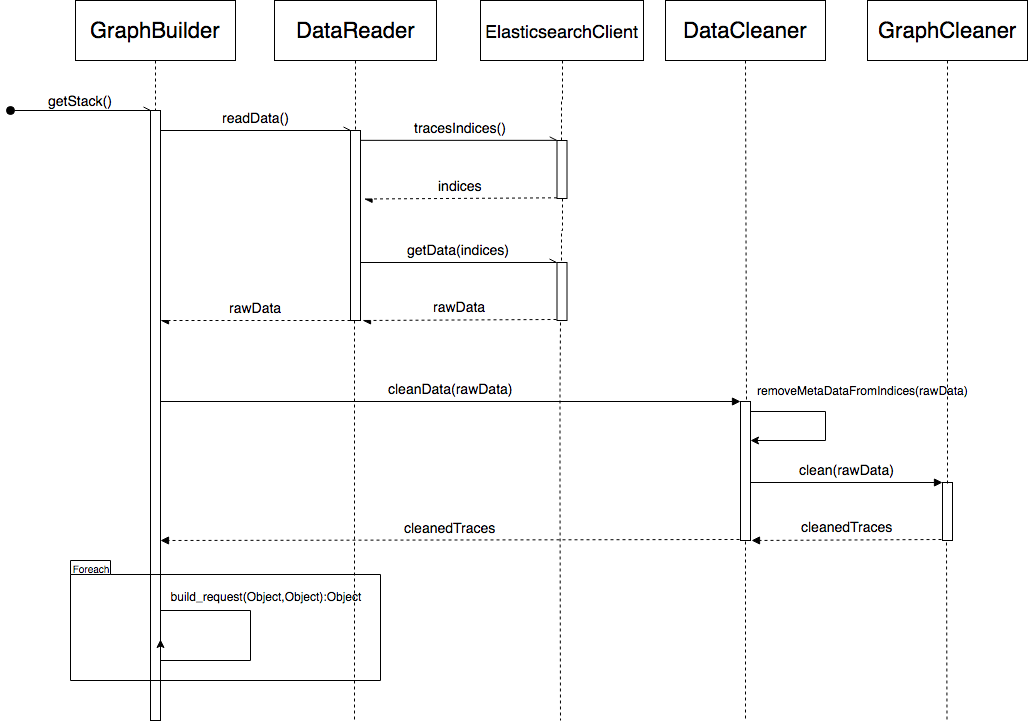
\includegraphics[width=1\textwidth]{Images/DiagrammaSequenzaStack.png}
	\caption{Diagramma di Sequenza UML rappresentante la costruzione della stack trace}
	\label{img:seqGraph}
\end{figure}
La sequenza di azioni per quanto riguarda l'interazione tra \texttt{StackBuilder}, \texttt{DataReader}, \texttt{ElasticsearchClient}, \texttt{DataCleaner} e \texttt{StackCleaner} è uguale a quella riguardande \texttt{GraphBuilder.}\\
Dopo aver ricevuto i dati e averli ripuliti dai dati superflui \texttt{StackBuilder} utilizza il metodo \texttt{build\_request()} per la costruzione delle richieste da visualizzare nella stack trace.


\section{Tracciamento dei requisiti}

\normalsize
\begin{longtable}{|c|c|c|}
	\hline
	\textbf{Codice Requisiti} & \textbf{Codice Use case} & \textbf{Implementazione} \\
	\hline
	\endhead
	R0F1 & UC1 & Implementato\\
	\hline
	R0F1.1 & UC1.1 & Implementato\\
	\hline
	R0F1.1.1 & UC1.5 & Implementato\\
	\hline
	R0F1.1.2 & UC1.6 & Implementato\\
	\hline
	R0F1.1.3 & UC1.7 & Non implementato\\
	\hline
	R1F1.2.1 & UC1.5.1 & Implementato\\
	\hline
	R1F1.2.2 & UC1.6.1 & Implementato\\
	\hline
	R1F1.2.3 & UC1.7.1 & Non implementato\\
	\hline
	R1F1.3 & UC1.2 & Implementato\\
	\hline
	R2F1.3.1 & UC1.2.2 & Non implementato\\
	\hline
	R1F1.3.2 & UC1.2.1 & Implementato\\
	\hline
	R1F1.4 & UC2 & Implementato\\
	\hline
	R2F1.4.1 & UC2.1 & Implementato\\
	\hline
	R2F1.4.2 & UC2.2 & Non implementato\\
	\hline
	R0F1.5 & UC1.3 & Implementato\\
	\hline
	R2F1.5.1 & UC1.3.2 & Implementato\\
	\hline
	R2F1.5.1.1 & UC1.3.5 & Non implementato\\
	\hline
	R2F1.5.1.2 & UC1.3.6 & Implementato\\
	\hline
	R0F1.5.2 & UC1.3.1 & Implementato\\
	\hline
	R0F1.5.2.1 & UC1.3.4 & Implementato\\
	\hline
	R0F1.5.2.2 & UC1.3.3 & Implementato\\
	\hline
	R1F1.6 & UC1.4 & Implementato\\
	\hline
	R1F1.6.1 & UC1.4.1 & Implementato\\
	\hline
	R1F1.6.2 & UC1.4.2 & Implementato\\
	\hline
	R1F1.6.2.1 & UC1.4.2.1 & Implementato\\
	\hline
	R1F1.6.2.2 & UC1.4.2.2 & Non implementato\\
	\hline
	R2F1.7 & UC3 & Implementato\\
	\hline
	R2F1.7.1 & UC3.1 & Implementato\\
	\hline
	R2F1.7.2 & UC3.2 & Implementato\\
	\hline
	R2F1.7.3 & UC3.3 & Non implementato\\
	\hline
	R1F1.8 & UC4 & Non implementato\\
	\hline
	R0F2 & UC5 & Implementato\\
	\hline
	R0F2.1 & UC5.1 & Implementato\\
	\hline
	R1F2.1.1 & UC5.1.1 & Implementato\\
	\hline
	R0F2.1.2 & UC5.1.2 & Implementato\\
	\hline
	R1F2.1.3 & UC5.1.3 & Implementato\\
	\hline
	R1F2.1.4 & UC5.1.4 & Implementato\\
	\hline
	R0F2.1.5 & UC5.1.5 & Implementato\\
	\hline
	R1F2.1.5.1 & UC5.1.5.1 & Non implementato\\
	\hline
	R1F2.2 & UC6 & Non implementato\\
	\hline
	R1F2.2.1 & UC7 & Non implementato\\
	\hline
	R1F2.2.1.1 & UC6.1 & Non implementato\\
	\hline
	R1F2.2.1.2 & UC6.2 & Non implementato\\
	\hline
	R1F2.2.2 & UC8 & Non implementato\\
	\hline
	R1F2.2.2.1 & UC6.1 & Non implementato\\
	\hline
	R1F2.2.2.2 & UC6.2 & Non implementato\\
	\hline
	R1F2.4 & UC9 & Non implementato\\
	\hline
	R0F3 & UC10 & Implementato\\
	\hline
	R0F3.1 & UC10.1 & Implementato\\
	\hline
	R0F3.1.1 & UC10.1.1 & Implementato\\
	\hline
	R1F3.1.2 & UC10.1.2 & Implementato\\
	\hline
	R1F3.1.3 & UC10.1.3 & Implementato\\
	\hline
	R2F3.1.4 & UC10.1.4 & Implementato\\
	\hline
	R2F3.2 & UC11 & Implementato\\
	\hline
	R2F3.2.1 & UC11.1 & Implementato\\
	\hline
	R2F3.2.2 & UC11.2 & Implementato\\
	\hline
	R1F4 & UC12 & Implementato\\
	\hline
	R1F4.1 & UC12.1 & Implementato\\
	\hline
	R1F4.1.1 & UC12.1.1 & Implementato\\
	\hline
	R1F4.1.2 & UC12.1.2 & Implementato\\
	\hline
	R1F4.1.3 & UC12.1.3 & Implementato\\
	\hline
	R1F4.1.4 & UC12.1.4 & Implementato\\
	\hline
	R1F4.1.5 & UC12.1.5 & Implementato\\
	\hline
	R1F4.2 & UC13 & Non implementato\\
	\hline
	R1F4.2.1 & UC14 & Non implementato\\
	\hline
	R1F4.2.1.1 & UC13.1 & Non implementato\\
	\hline
	R1F4.2.1.2 & UC13.2 & Non implementato\\
	\hline
	R1F4.2.2 & UC15 & Non implementato\\
	\hline
	R1F4.2.2.1 & UC13.1 & Non implementato\\
	\hline
	R1F4.2.2.2 & UC13.2 & Non implementato\\
	\hline
	\caption[Tracciamento Requisiti-Use case]{Tracciamento Requisiti-Use case}
\end{longtable}
\clearpage
\normalsize
\begin{longtable}{|c|c|c|}
	\hline
	\textbf{Codice Use case} & \textbf{Codice Requisiti} & \textbf{Implementazione} \\
	\hline
	\endhead
	UC1 & R0F1 & Implementato\\
	\hline
	UC1.1 & R0F1.1 & Implementato\\
	\hline
	UC1.2 & R1F1.3 & Implementato\\
	\hline
	UC1.2.1 & R1F1.3.2 & Implementato\\
	\hline
	UC1.2.2 & R2F1.3.1 & Non implementato\\
	\hline
	UC1.3 & R0F1.5 & Implementato\\
	\hline
	UC1.3.1 & R0F1.5.2 & Implementato\\
	\hline
	UC1.3.2 & R2F1.5.1 & Implementato\\
	\hline
	UC1.3.3 & R0F1.5.2.2 & Implementato\\
	\hline
	UC1.3.4 & R0F1.5.2.1 & Implementato\\
	\hline
	UC1.3.5 & R2F1.5.1.1 & Non implementato\\
	\hline
	UC1.3.6 & R2F1.5.1.2 & Implementato\\
	\hline
	UC1.4 & R1F1.6 & Implementato\\
	\hline
	UC1.4.1 & R1F1.6.1 & Implementato\\
	\hline
	UC1.4.2 & R1F1.6.2 & Implementato\\
	\hline
	UC1.4.2.1 & R1F1.6.2.1 & Implementato\\
	\hline
	UC1.4.2.2 & R1F1.6.2.2 & Non implementato\\
	\hline
	UC1.5 & R0F1.1.1 & Implementato\\
	\hline
	UC1.5.1 & R1F1.2.1 & Implementato\\
	\hline
	UC1.6 & R0F1.1.2 & Implementato\\
	\hline
	UC1.6.1 & R1F1.2.2 & Implementato\\
	\hline
	UC1.7 & R0F1.1.3 & Non implementato\\
	\hline
	UC1.7.1 & R1F1.2.3 & Non implementato\\
	\hline
	UC2 & R1F1.4 & Implementato\\
	\hline
	UC2.1 & R2F1.4.1 & Implementato\\
	\hline
	UC2.2 & R2F1.4.2 & Non implementato\\
	\hline
	UC3 & R2F1.7 & Implementato\\
	\hline
	UC3.1 & R2F1.7.1 & Implementato\\
	\hline
	UC3.2 & R2F1.7.2 & Implementato\\
	\hline
	UC3.3 & R2F1.7.3 & Non implementato\\
	\hline
	UC4 & R1F1.8 & Non implementato\\
	\hline
	UC5 & R0F2 & Implementato\\
	\hline
	UC5.1 & R0F2.1 & Implementato\\
	\hline
	UC5.1.1 & R1F2.1.1 & Implementato\\
	\hline
	UC5.1.2 & R0F2.1.2 & Implementato\\
	\hline
	UC5.1.3 & R1F2.1.3 & Implementato\\
	\hline
	UC5.1.4 & R1F2.1.4 & Implementato\\
	\hline
	UC5.1.5 & R0F2.1.5 & Implementato\\
	\hline
	UC5.1.5.1 & R1F2.1.5.1 & Non mplementato\\
	\hline
	UC6 & R1F2.2 & Non implementato\\
	\hline
	UC6.1 & R1F2.2.1.1 & Non implementato\\
	& R1F2.2.2.1 & \\
	\hline
	\clearpage
	UC6.2 & R1F2.2.1.2 & Non implementato\\
	& R1F2.2.2.2 & \\
	\hline
	UC7 & R1F2.2.1 & Non implementato\\
	\hline
	UC8 & R1F2.2.2 & Non implementato\\
	\hline
	UC9 & R1F2.4 & Non implementato\\
	\hline
	UC10 & R0F3 & Implementato\\
	\hline
	UC10.1 & R0F3.1 & Implementato\\
	\hline
	UC10.1.1 & R0F3.1.1 & Implementato\\
	\hline
	UC10.1.2 & R1F3.1.2 & Implementato\\
	\hline
	UC10.1.3 & R1F3.1.3 & Implementato\\
	\hline
	UC10.1.4 & R2F3.1.4 & Implementato\\
	\hline
	UC11 & R2F3.2 & Implementato\\
	\hline
	UC11.1 & R2F3.2.1 & Implementato\\
	\hline
	UC11.2 & R2F3.2.2 & Implementato\\
	\hline
	UC12 & R1F4 & Implementato\\
	\hline
	UC12.1 & R1F4.1 & Implementato\\
	\hline
	UC12.1.1 & R1F4.1.1 & Implementato\\
	\hline
	UC12.1.2 & R1F4.1.2 & Implementato\\
	\hline
	UC12.1.3 & R1F4.1.3 & Implementato\\
	\hline
	UC12.1.4 & R1F4.1.4 & Implementato\\
	\hline
	UC12.1.5 & R1F4.1.5 & Implementato\\
	\hline
	UC13 & R1F4.2 & Non implementato\\
	\hline
	UC13.1 & R1F4.2.1.1 & Non implementato\\
	& R1F4.2.2.1 &\\
	\hline
	UC13.2 & R1F4.2.1.2 & Non implementato\\
	& R1F4.2.2.2 &\\
	\hline
	UC14 & R1F4.2.1 & Non implementato\\
	\hline
	UC15 & R1F4.2.2 & Non implementato\\
	\hline
	\caption[Tracciamento Use case-Requisiti]{Tracciamento Use case-Requisiti}
\end{longtable}
\clearpage
